\documentclass{article}
\usepackage{amsmath}
\usepackage{graphicx}

\begin{document}
\section{Light Incident on a Simple Boundary}
    \begin{figure}
        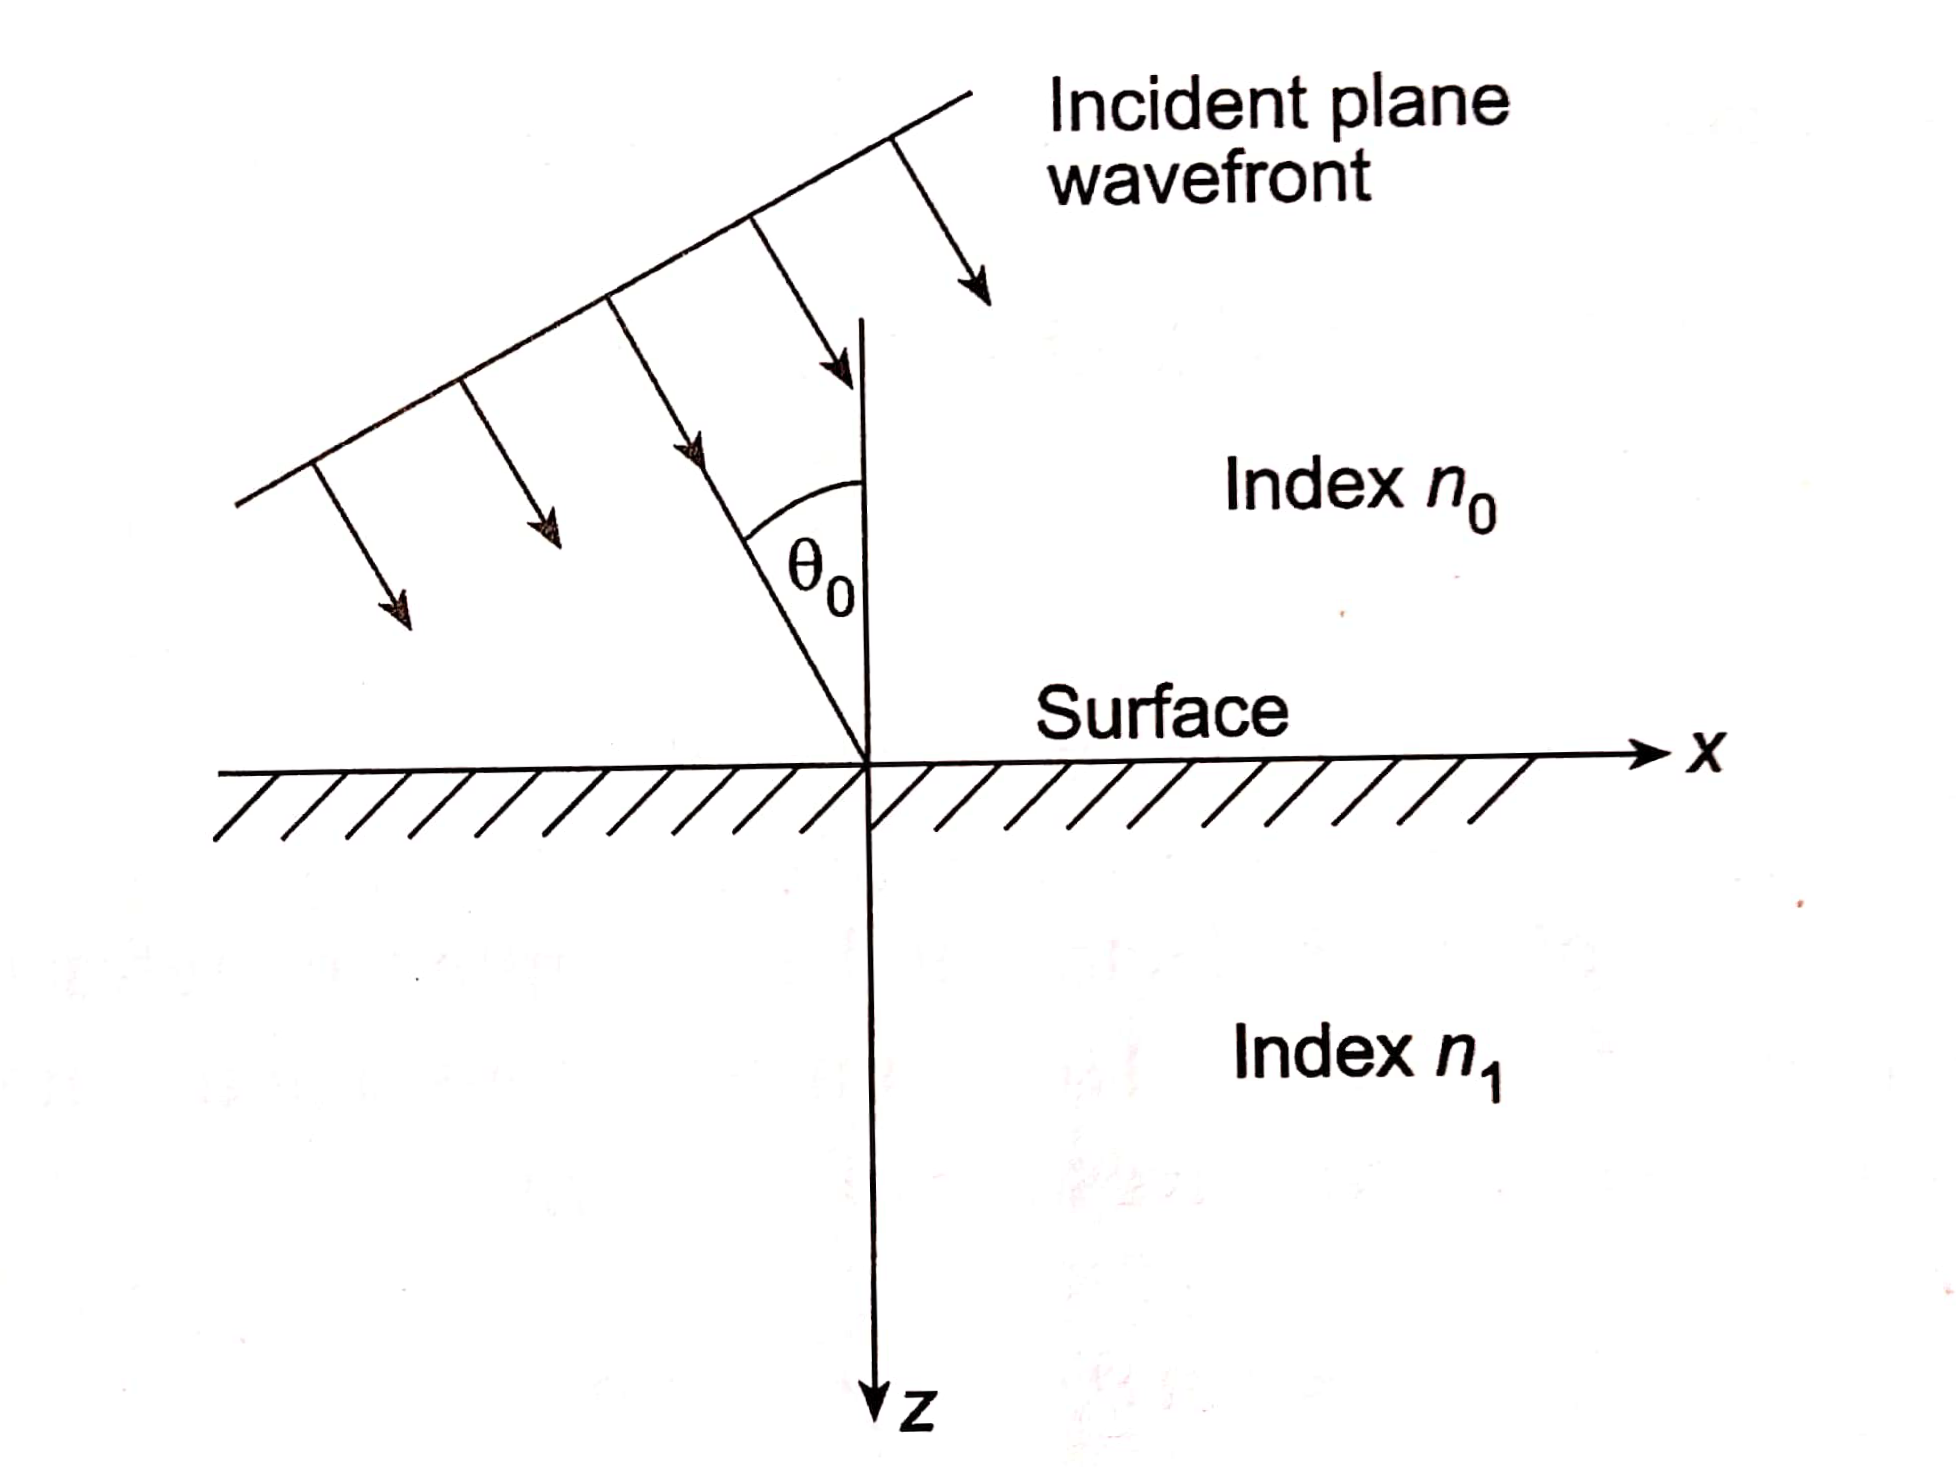
\includegraphics[width=\linewidth]{simple_boundary.png}
        \caption{Simple Boundary}
        \label{fig:simp}
    \end{figure}
    For an electromagnetic wave incident on a surface from index of refraction $n_0$ to $n_1$ at an angle $\theta_0$, the phase factors are given by
    \begin{align}
        &\text{Incident Wave} & &\mathrm{exp}\left\{ i [\omega t - (2\pi n_0 / \lambda)(x \sin \theta_0 - z \cos \theta_0)]\right\} \\
        &\text{Reflected Wave} & &\mathrm{exp}\left\{ i [\omega t - (2\pi n_0 / \lambda)(\alpha_r x + \beta_r y + \gamma_r z)]\right\} \\
        &\text{Transmitted Wave} & &\mathrm{exp}\left\{ i [\omega t - (2\pi n_1 / \lambda)(\alpha_t x + \beta_t y + \gamma_t z)]\right\}
    \end{align}
    This situation is schematically shown in Figure \ref{fig:simp}

    Let us temporarily consider light normally incident on the boundary. The electric field will be aligned along the positive x-direction, requiring the the magnetic field to be aligned along the positive y-axis. We apply the boundary conditions:
    \begin{enumerate}
        \item Electric field vector continuous across boundary
        \begin{equation}
            E_i + E_r = E_t
        \end{equation} 
        \item Magnetic field vector continuous across boundary
        \begin{equation}
            H_i - H_r = H_t
            \label{eq:magcont}
        \end{equation}
    \end{enumerate}
    Figure \ref{fig:norm} pictorially shows these conditions.

    \begin{figure}
        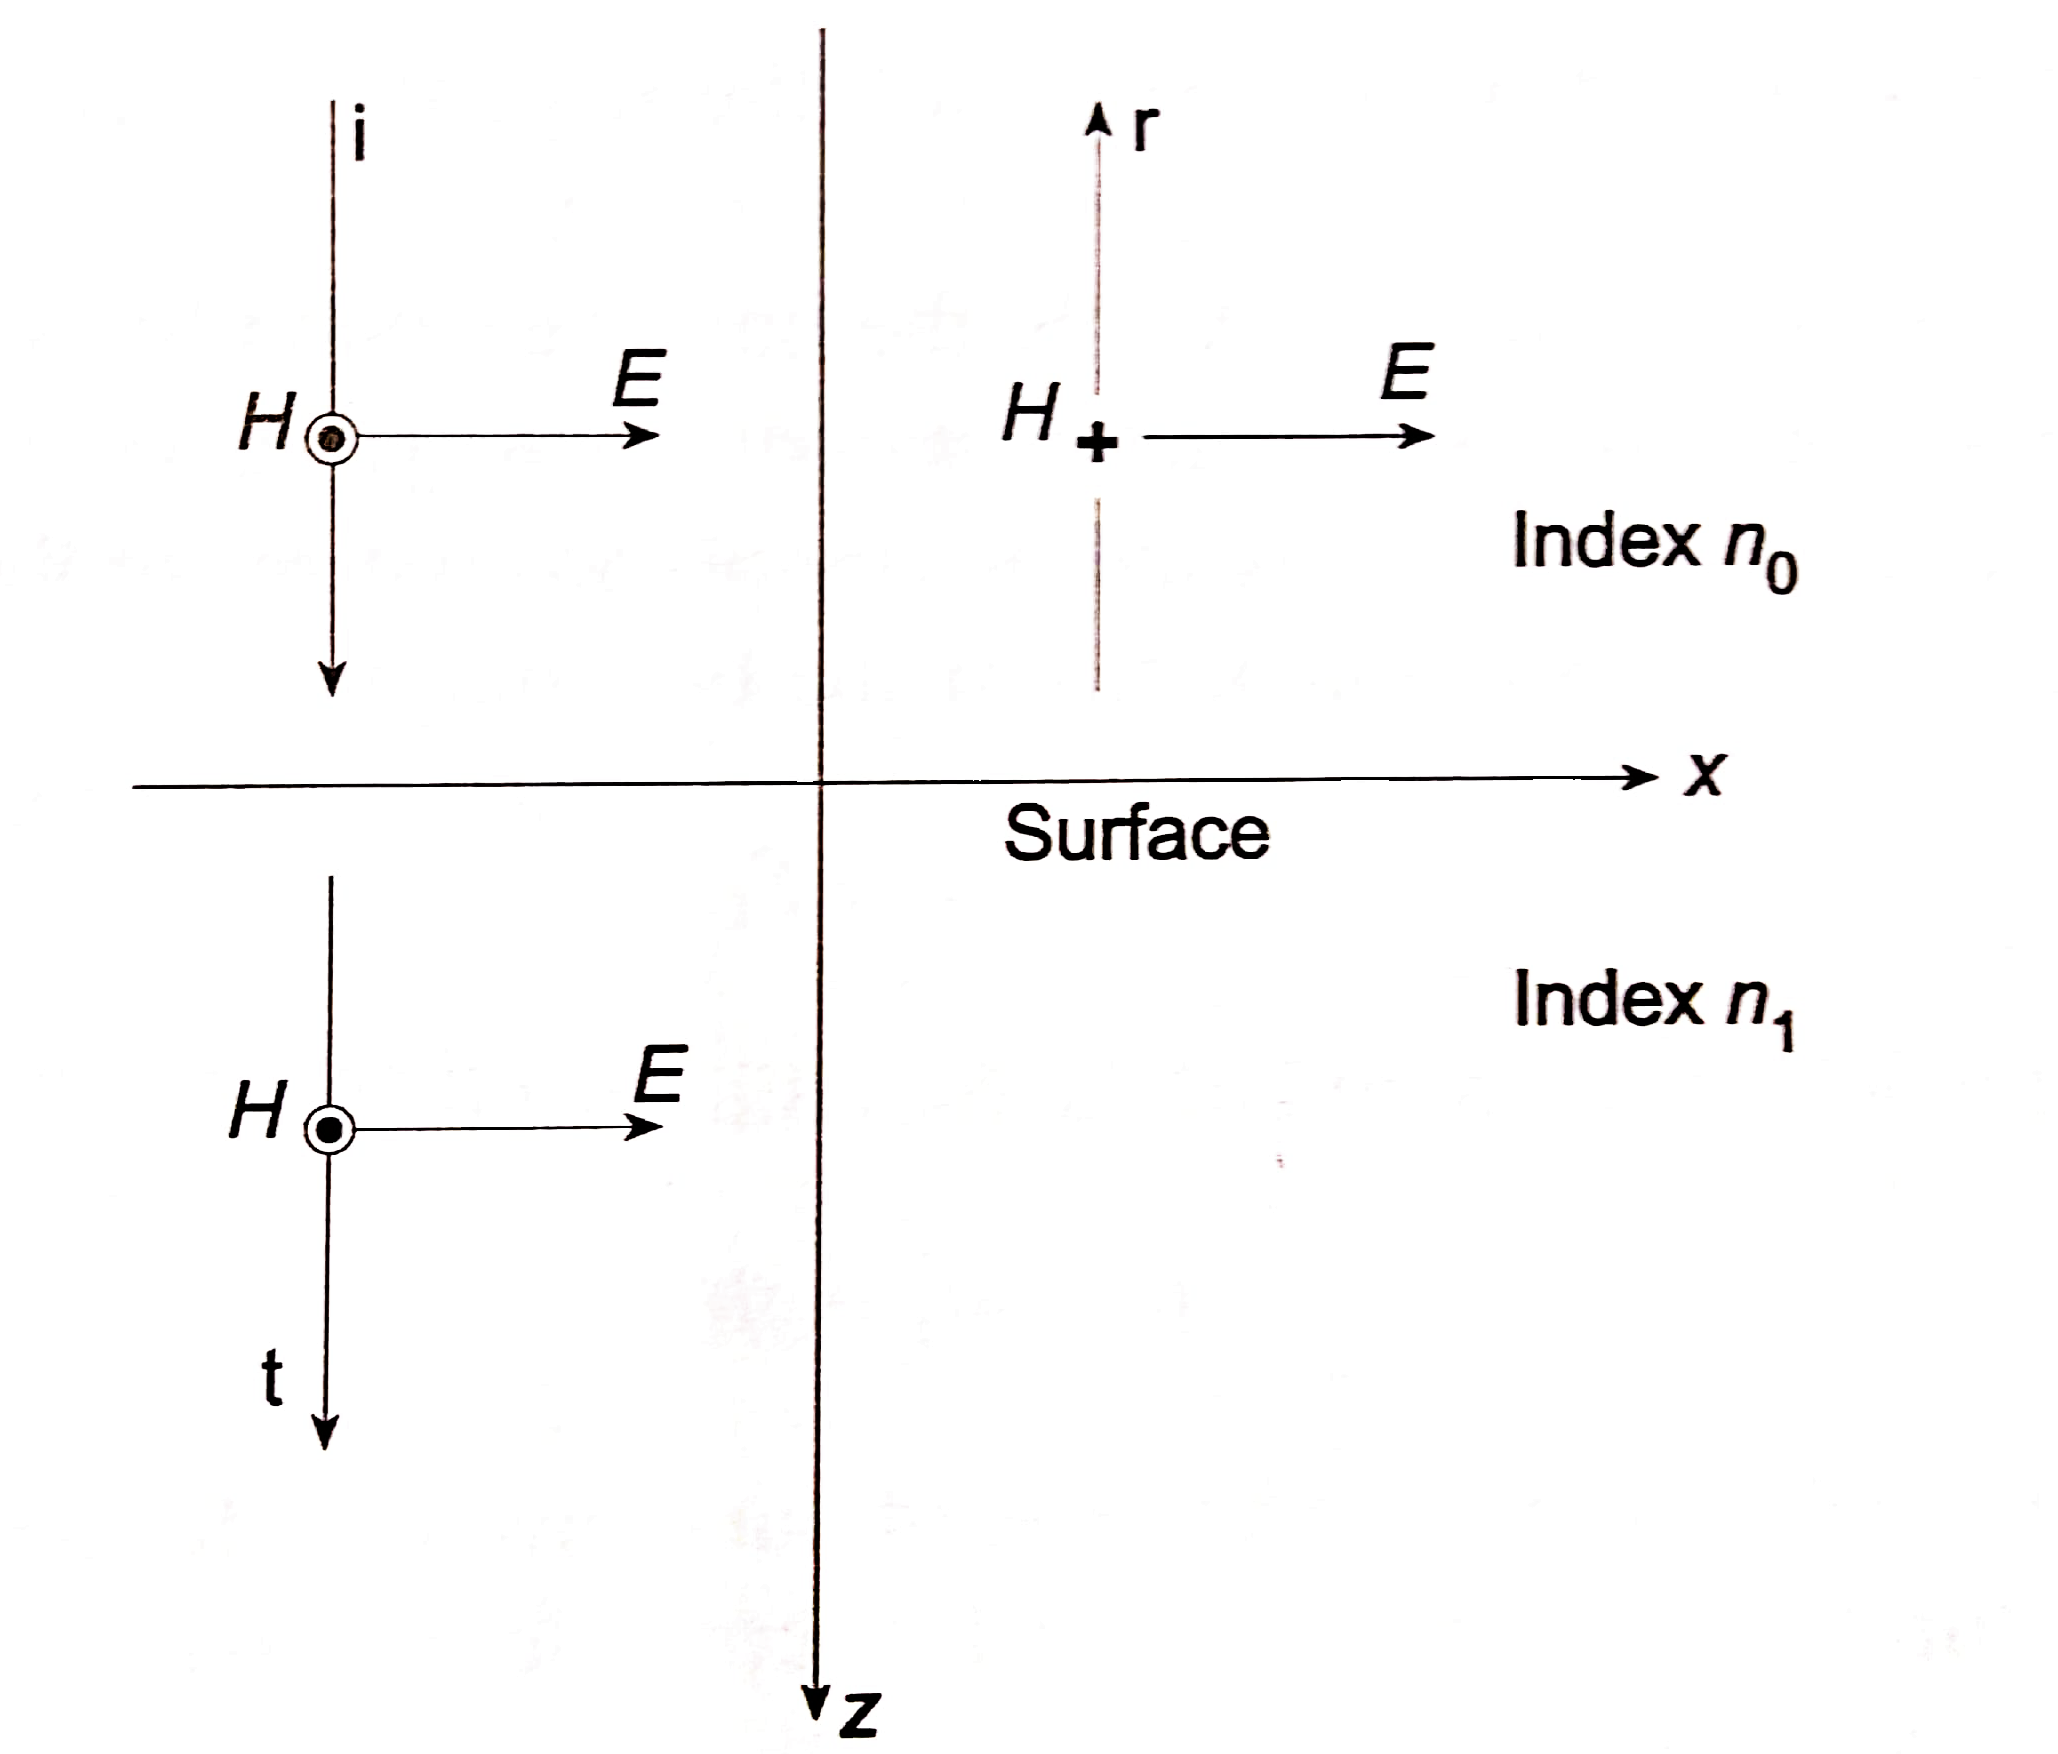
\includegraphics[width=\linewidth]{simple_boundary_normal.png}
        \caption{Light Normally incident on surface with electric and magnetic vectors shown}
        \label{fig:norm}
    \end{figure}

    Using the characteristic admittance, $y$, of each layer, Equation \ref{eq:magcont} can be expressed as

    \begin{equation}
        y_0 E_i - y_0 E_r = y_1 E_t
    \end{equation}

    We can then compute the reflection coefficient $\rho$ and the transmission coefficient $\tau$
    \begin{align}
        \rho &= \frac{E_r}{E_i} = \frac{y_0 - y_1}{y_0 + y_1} = \frac{n_0 - n_1}{n_0 + n_1} \\
        \tau &= \frac{E_t}{E_i} = \frac{2 y_0}{y_0 + y_1} = \frac{2 n_0}{n_0+n_1}
    \end{align}
    Where the last equality comes about since in the optical regime
    $$ y = n y_{\mathrm{vaccuum}} $$

    And finally, we compute the transmittance $T$ and reflectance $R$ by
    \begin{align}
        T &= \frac{y_1}{y_0}\tau^2 = \frac{4 n_0 n_1}{(n_0 + n_1)^2} \label{eq:trans} \\
        R &= \rho^2 = \left(\frac{n_0 - n_1}{n_0 + n_1}\right)^2 \label{eq:reflec}
    \end{align}

    As expected for a non-absorbing medium $$ T + R = 1 $$

    To extend this analysis to oblique incidence, we introduce the tilted optical admittance $\eta$ which connects the components of the electric and magnetic fields parallel to the boundary
    \begin{equation}
        \eta = \frac{H^{\parallel}}{E^{\parallel}}
    \end{equation}
    Using this tilted admittance, the transmission and reflection coefficients can be computed the same way they are computed in equations \ref{eq:trans} and \ref{eq:reflec}.

    It is worthy to note that to calculating $\eta$ depends on the polarization of incident light. In the case of s and p-polarization, the tilted admittances become
    \begin{align}
        \eta_p &= y/\cos \theta \\
        \eta_s &= y \cos \theta
    \end{align}
    This will be of little importance in the upcoming analysis.

\section{Transmission through a Thin Film}
    We turn our attention to the geometry seen in Figure \ref{fig:film}. We first consider the tangential components of the electric and magnetic fields at boundary b, while introducing the notation $+$ referring to the positive-travelling wave and $-$ referring to waves traveling in the opposite direction.
    \begin{align}
        E_b &= E_{1b}^+ + E_{1b}^- \\
        H_b &= \eta_1 E_{1b}^+ - \eta_1 E_{1b}^-    
    \end{align}
    \begin{figure}
        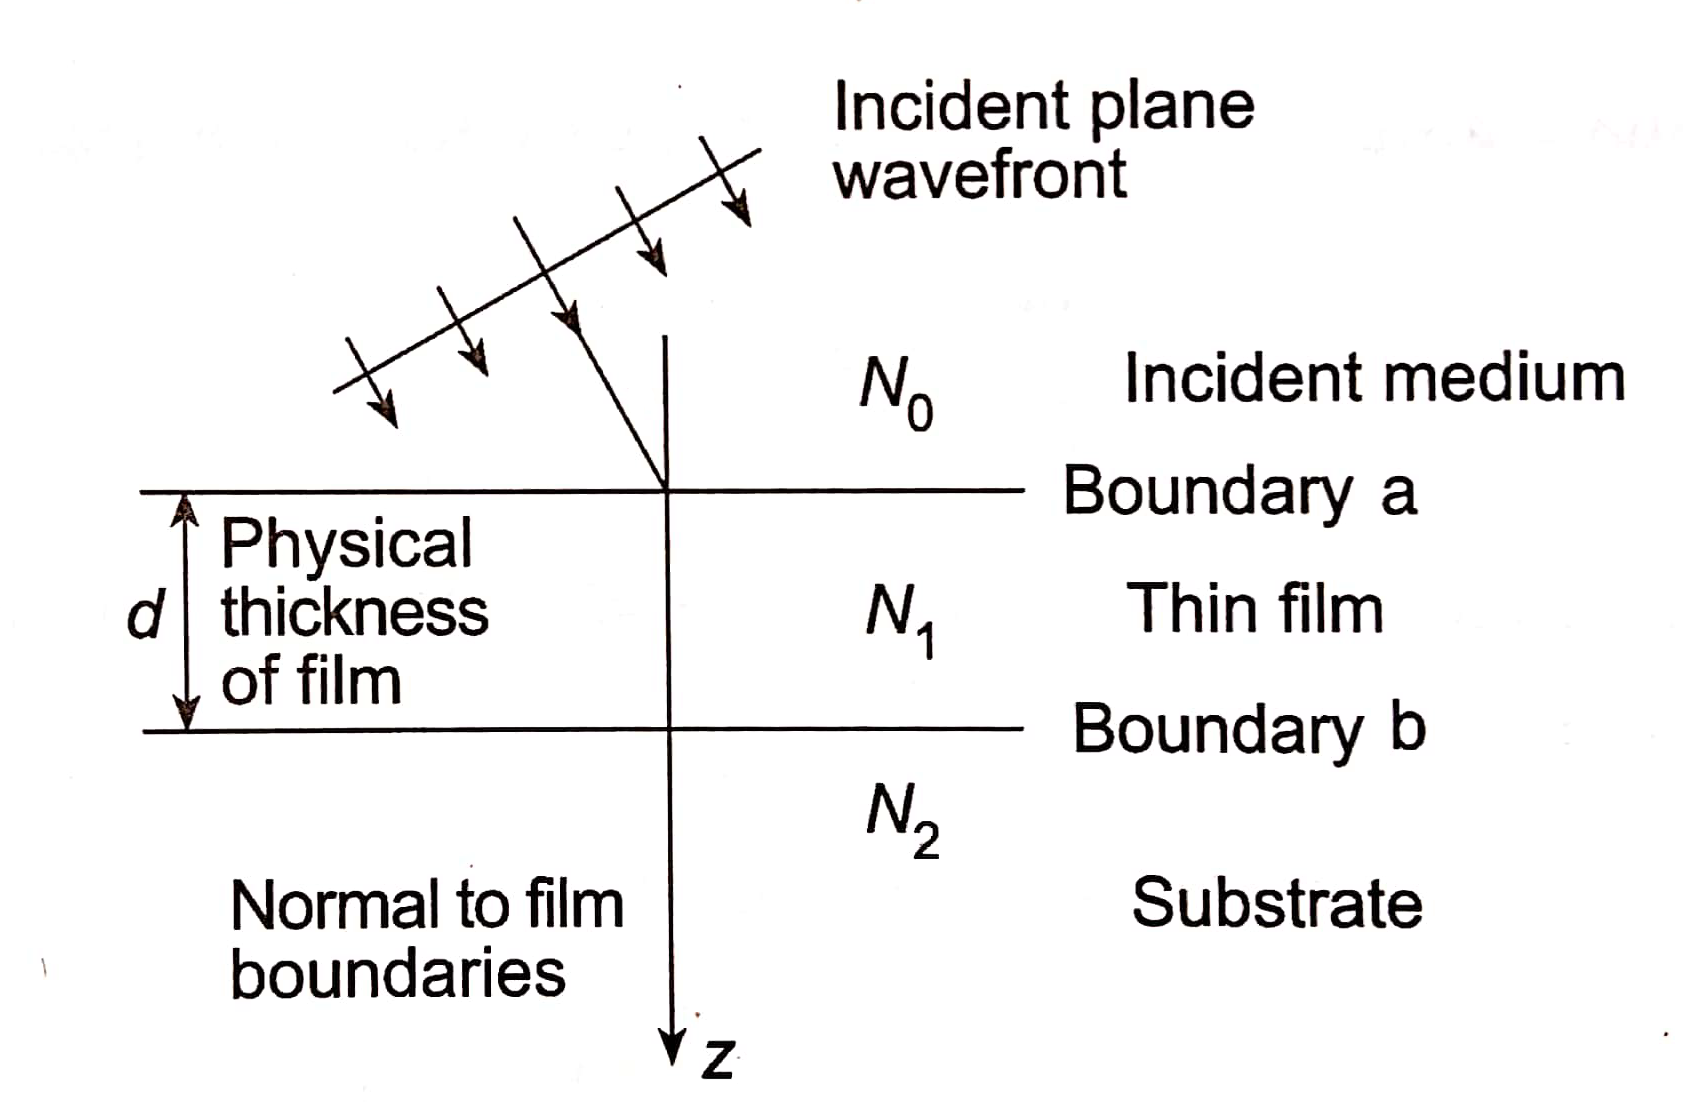
\includegraphics[width=\linewidth]{thin_film.png}
        \caption{Plane wave incident on a thin film}
        \label{fig:film}
    \end{figure}
    We can find the fields at the interface at $a$ by considering the phase difference at the same time, across the change in the $z$ coordinate by $-d$. We say that the positive going wave will be multiplied by $e^{i \delta}$ while the negative going wave will be multiplied by $e^{-i \delta}$ where
    \begin{equation}
        \delta = 2 \pi N_1 d \cos \theta_1 / \lambda    
    \end{equation}
    $N$ is the complex analogue to the refractive index $n$ and is given by $$N = n - ik $$ where $k$ is the extinction coefficient. For our analysis, we are assuming non-absorbing media, and the distinction between $N$ and $n$ can be ignored.
    
    With these tools, we can relate $E_a$ and $H_a$ to $E_b$ and $H_b$ by the matrix equation
    \begin{equation}
        \label{eq:charmatrix}
        \begin{bmatrix}
            E_a \\
            H_a
        \end{bmatrix}
        =
        \begin{bmatrix}
            \cos \delta & (i \sin \delta)/\eta_1 \\
            i \eta_1 \sin \delta & \cos \delta
        \end{bmatrix}
        \begin{bmatrix}
            E_b \\
            H_b
        \end{bmatrix}        
    \end{equation}
\end{document}